%%-------------------------------------------------------------------------------------- Início
\begin{frame}[allowframebreaks, t, fragile]{Associações em Rails}
	\begin{itemize}
		\item O gerador \verb|scaffold| utiliza por padrão o ActiveRecord. Isto significa:
		\begin{itemize}
			\item Tabelas para postagens e comentários foram criadas quando executamos as migrações
			\item Um conexão com o banco de dados é estabelecida
			\item O ORM é configurado para as postagens e comentátios foi criado - o "M" do
			MVC.
		\end{itemize}

		\item No entanto, uma coisa está faltando:
		\begin{itemize}
			\item  \alert{tem-se que assegurar que qualquer
				comentários sejam associados às suas postagens}
		\end{itemize}

		\item Para tornar os modelos em Rails totalmente funcionais precisamos adicionar
		\alert{associações}:
		\begin{itemize}
			\item cada postagem precisa saber os comentários associado a ele
			\item cada comentário precisa saber qual é a postagem ele pertence
		\end{itemize}
	
		\item Há uma relação \alert{muitos-para-um} entre comentários e postagens
		uma:
		\begin{figure}[h!]
			\centering
			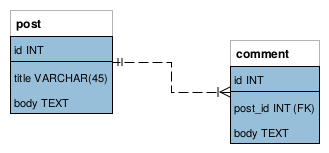
\includegraphics[width=0.70\textwidth]{imagens/modelo-de-dados-blog.png}
		\end{figure}
		
		\item O ActiveRecord contém um conjunto de métodos de classe para
		\alert{vinculação} de objetos por meio de \alert{chaves estrangeiras}
		
		\item Para habilitar isto, deve-se declarar as \alert{associações} dentro dos modelos
		usando:
		\begin{table}[tp] 
			\scriptsize 
			\setlength{\tabcolsep}{8pt}
			\setlength{\extrarowheight}{2pt}   			
			\begin{tabular}{|l|l|l|} 
				\hline
				\textbf{Associação} & \textbf{Modelo Pai} & \textbf{Modelo Filho}\\
				\hline
				Um-para-um & \verb|has_one| & \verb|belongs_to| \\
				\hline
				Muitos-para-um & \verb|has_many| & \verb|belongs_to| \\
				\hline
				Muitos-para-muitos & \verb|has_and_belongs_to_many| & *na tabela junção \\
				\hline
			\end{tabular}
		\end{table}
		
	\end{itemize}	
\end{frame}